% Created 2013-05-23 Thu 12:10
\documentclass[presentation,t,hideothersubsections]{beamer}
\usepackage[utf8]{inputenc}
\usepackage[T1]{fontenc}
\usepackage{fixltx2e}
\usepackage{graphicx}
\usepackage{longtable}
\usepackage{float}
\usepackage{wrapfig}
\usepackage{soul}
\usepackage{textcomp}
\usepackage{marvosym}
\usepackage{wasysym}
\usepackage{latexsym}
\usepackage{amssymb}
\usepackage{amstext}
\usepackage{hyperref}
\tolerance=1000
     \usepackage{listings}
\usepackage{xcolor}
\usepackage[frenchb,]{babel}
     \RequirePackage{xcolor}
\definecolor{mc@lstidentifier}{HTML}{000000} % black
\definecolor{mc@lstcomment}{HTML}{FF0000} % red
\definecolor{mc@lststring}{HTML}{008000} % dark green
\definecolor{mc@lstkeyword}{HTML}{0000FF} % blue
\definecolor{mc@lstbackground}{HTML}{FFFFCC} % light yellow
\definecolor{mc@lstframe}{HTML}{FFEE88} % dark yellow
\lstdefinelanguage{org}{%
morekeywords={:results, :session, :var, :noweb, :exports},
sensitive=false,
morestring=[b]",
morecomment=[l]{\#},
}
\lstdefinelanguage{dot}{%
morekeywords={graph},
sensitive=false,
}
\lstset{%
lineskip=-0.1em,
%
basicstyle=\ttfamily\scriptsize, % font that is used for the code
identifierstyle=\color{mc@lstidentifier},
commentstyle=\color{mc@lstcomment}\itshape,
stringstyle=\color{mc@lststring},
keywordstyle=\color{mc@lstkeyword},
%
extendedchars=false,
inputencoding=utf8,
upquote, %
tabsize=4, % set default tabsize to 4 spaces
showtabs=false, % show tabs within strings adding particular underscores
%  tab=$\to$,
showspaces=false, % show spaces adding particular underscores
showstringspaces=false, % underline spaces within strings
%
numbers=left, % where to put the line numbers
stepnumber=0, % step between two line numbers
numberstyle=\tiny, % line number font size
%
captionpos=b, % set the caption position to `bottom'
%
xleftmargin=0.4em, % text to the right
xrightmargin=0.4em, % text to the left
breaklines=false, % don't break long lines of code
%
frame=single, % add a frame around the code
framexleftmargin=0pt, % frame back to the left
framexrightmargin=0pt, % frame back to the right
backgroundcolor=\color{mc@lstbackground}, % set the background color
rulecolor=\color{mc@lstframe}, % frame color
%
columns=flexible, % try not to ruin the spacing intended by the font designer
keepspaces=true, % don't drop spaces to fix column alignment
%
% mathescape, % allow escaping to (La)TeX mode within $..$
escapechar=², % allow escaping to (La)TeX mode within ²..²
% The backquote was NOT judicious: in some code (comments), I wrap vars
% between such a backquote (`var')
%
% conversion of UTF-8 chars to latin1
literate=
{á}{{\'a}}1
{à}{{\`a}}1
{â}{{\^a}}1
{ä}{{\"a}}1
{é}{{\'e}}1
{è}{{\`e}}1
{ê}{{\^e}}1
{ë}{{\"e}}1
{í}{{\'i}}1
{ì}{{\`i}}1
{î}{{\^i}}1
{ï}{{\"i}}1
{ó}{{\'o}}1
{ò}{{\`o}}1
{ô}{{\^o}}1
{ö}{{\"o}}1
{ú}{{\'u}}1
{ù}{{\`u}}1
{û}{{\^u}}1
{ü}{{\"u}}1
}
\usepackage{tikz}
\usepackage{pgfplots}
% must be loaded after url and hyperref
\RequirePackage[colorinlistoftodos]{todonotes}% (not in medium TeX Live installation)
\definecolor{mc@todobg}{HTML}{F5F5F5} % white smoke
\definecolor{mc@todoborder}{HTML}{DDDDDD} % ~ gray87
\renewcommand{\@todonotes@backgroundcolor}{mc@todobg}
\renewcommand{\@todonotes@bordercolor}{mc@todoborder}
%the needed packages
\usepackage[absolute,showboxes,overlay]{textpos}
%\TPshowboxestrue % commenter une fois fini
\TPshowboxesfalse % décommenter pour faire disparaitre les boites
\textblockorigin{10mm}{10mm} % origine des positions
%adjust the TPHorizModule and TPHorizModule units to the displayed mm %grid
\TPGrid{210}{297}
%puts a graphic at the absolute position described by the grid
%#1 x, #2 y, #3 width, #4 height, #5 graphic
\newcommand\putpic[5]{%
\begin{textblock}{#3}(#1,#2)
\includegraphics[width=#3\TPHorizModule,
height=#4\TPVertModule]{#5}
\end{textblock}
}
\logo{
\includegraphics[height=2cm]{org-mode-unicorn}}
\usepackage[frenchb]{babel}
\usepackage{multicol}
\usetheme{mc}
\author{Fabrice Niessen}
\date{2012-06-13}
\title{Org mode pour LaTeXiens}
\hypersetup{
  pdfkeywords={stage, latex, org mode, dunkerque},
  pdfsubject={Tout ce que vous avez toujours voulu savoir sur Org},
  pdfcreator={Emacs 24.3.1 (Org mode 8.0.3)}}
\begin{document}

\maketitle
\begin{frame}{Plan}
\tableofcontents
\end{frame}



\section{Introduction}
\label{sec-1}

\subsection{\LaTeX{}}
\label{sec-1-1}

\begin{frame}[label=sec-1-1-1]{\LaTeX{}}
\begin{itemize}
\item Documents ou présentations avec un rendu de haute qualité

\item Versions successives faciles à comparer grâce à, par exemple,
\begin{itemize}
\item Diff de CVS, SVN Git ou
\item Ediff (Diff interactif)
\end{itemize}

\item Syntaxe pénible pour écrire des tableaux ou pour gérer des listes
imbriquées

\item Difficultés à convaincre vos collègues de passer à \LaTeX{}
\end{itemize}
\end{frame}
\subsection{Org mode}
\label{sec-1-2}

\begin{frame}[label=sec-1-2-1]{Définition}
\begin{itemize}
\item \alert{Org mode}, [awr-g mohd], \emph{noun}; \\
  \emph{Emacs major mode for note-taking, project planning, and authoring.}
\end{itemize}

\pause

%\putpic{20}{20}{100}{100}{Carsten.png}

%\begin{textblock*}{30mm}[0,0](180mm,40mm)
\begin{textblock*}{10mm}[0,0](0.92\textwidth,22mm)
    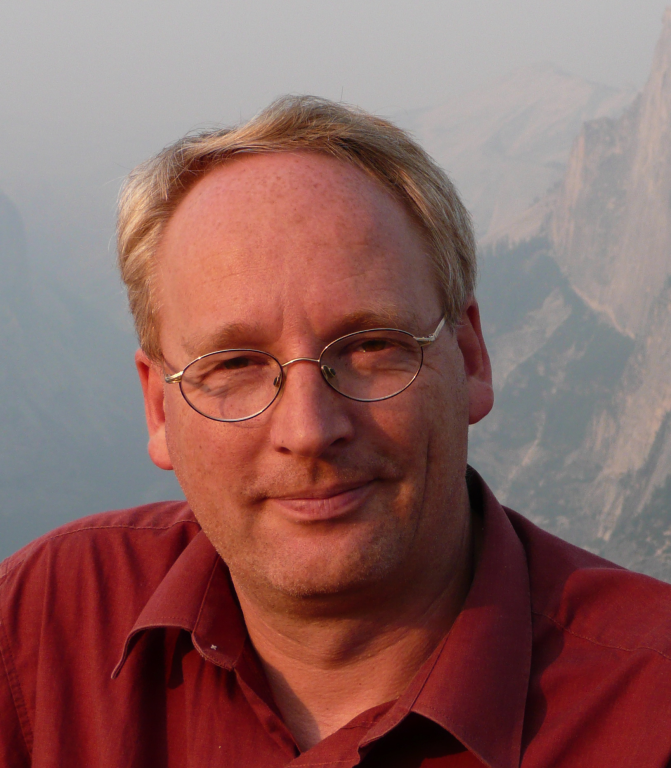
\includegraphics[width=17mm]{Carsten.png}
\end{textblock*}

\#\#+ATTR\_$\backslash$LaTeX\{\}: width=1.7cm
\#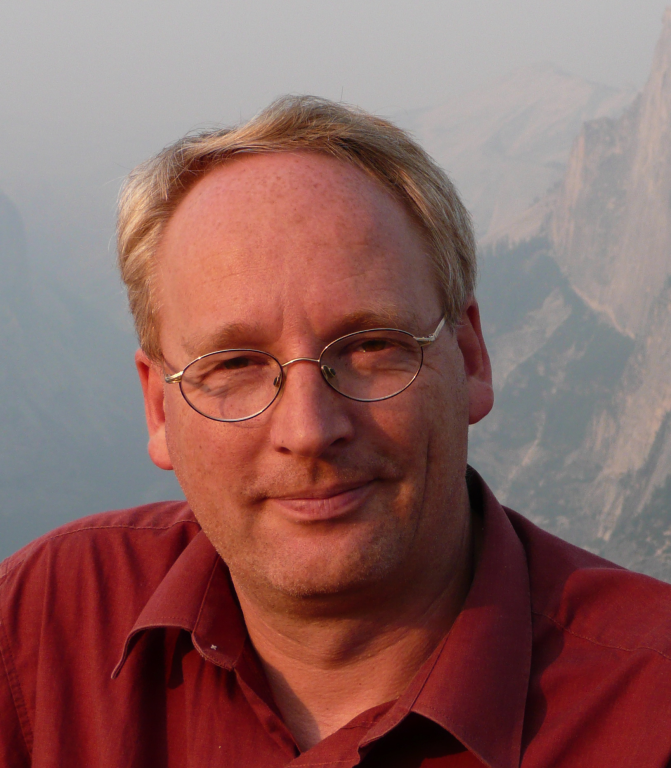
\includegraphics[width=.9\linewidth]{Carsten.png}

\begin{itemize}
\item Créé en 2003 par Carsten Dominik
\begin{itemize}
\item Principal développeur et architecte jusqu'en fin 2010
\item Repris par Bastien Guerry
\end{itemize}

\item \href{http://orgmode.org/worg/org-tutorials/org-screencasts/org-mode-google-tech-talk.html}{Google Tech Talk} du 15 juillet 2008
\end{itemize}

\begin{quote}
"Org mode does outlining, note-taking, hyperlinks, spreadsheets, TODO lists,
project planning, GTD, HTML and \LaTeX{} authoring, all with plain text files in
Emacs." -- Carsten Dominik
\end{quote}
\end{frame}
\begin{frame}[label=sec-1-2-2]{Org mode}
\begin{itemize}
\item \alert{Balisage} virtuellement nul, syntaxe "à la Wiki" \alert{très lisible} (aussi facile à
lire que du texte brut)

\item \alert{Rédaction} d'un document ou d'une présentation aussi \alert{simple} que l'écriture
d'un \emph{email}

\item Fantastique éditeur de \alert{listes} et de \alert{tables} (disponible en mode mineur)

\item Difficultés à convaincre vos collègues de passer à\ldots{} Emacs\footnote{Evil = émulateur Vim pour Emacs}
\end{itemize}
\end{frame}
\begin{frame}[label=sec-1-2-3]{Org mode \\ Possibilités supplémentaires par rapport à \LaTeX{}}
\begin{itemize}
\item \emph{Outlining} \footnote{Résumé hiérarchique des idées principales d'un sujet}
\item Tableur
\item Statut (TODO / DONE) et \emph{tags} sur les sections
\item Export vers HTML (site Web), LibreOffice, etc.
\item Fonctions de recherche avancée
\item \ldots{}
\end{itemize}

\begin{quote}
At its core, Org mode is a simple outliner for \alert{note-taking} and \alert{[task] list
management}. You can learn the basics for using it in five minutes. This may
be all you need, and Org mode will not impose more complex features on you.
-- \url{http://orgmode.org/}
\end{quote}
\end{frame}
\section{Structuration}
\label{sec-2}

\subsection{Fichier}
\label{sec-2-1}

\begin{frame}[fragile,label=sec-2-1-1]{Fichier \\ Généralités}
 \begin{itemize}
\item Extension du nom de fichier~: \texttt{.org}
\item Codage (\texttt{latin1}, \texttt{utf8}) auto-détecté
\item Codage \texttt{T1} (= défaut) pour l'accès aux \emph{glyphes} des fontes
\end{itemize}
\end{frame}
\begin{frame}[fragile,label=sec-2-1-2]{Fichier \\ Classes}
 \begin{itemize}
\item Classes connues dans la liste \texttt{org-export-latex-classes}
\begin{itemize}
\item \texttt{article}
\item \texttt{report}
\item \texttt{book}
\item \texttt{beamer}
\end{itemize}

\item Classe par défaut dans la variable \texttt{org-export-latex-default-class}
\begin{itemize}
\item \texttt{article}
\end{itemize}

\item Paramétrage dans un fichier
\end{itemize}

\lstset{language=org,numbers=none}
\begin{lstlisting}
#+LaTeX_CLASS: report
#+LaTeX_CLASS_OPTION: [12pt]
\end{lstlisting}
\end{frame}
\subsection{Packages}
\label{sec-2-2}

\begin{frame}[fragile,label=sec-2-2-1]{Packages par défaut \\ Packages insérés dans chaque en-tête \LaTeX{}}
 \begin{itemize}
\item \texttt{org-export-latex-default-packages-alist}
\begin{itemize}
\item \texttt{inputenc}, \texttt{fontenc} pour la sélection des types de caractères et de fontes
\item \texttt{textcomp}, \texttt{marvosymb}, \texttt{wasysym}, \texttt{latexsym}, \texttt{amssym} pour les divers symboles
\item \texttt{graphicx} pour l'inclusion d'images
\item \texttt{float}, \texttt{wrapfig} pour le placement des figures
\item \texttt{longtable} pour les longues tables
\item \texttt{hyperref} pour les références croisées
\end{itemize}

\item \texttt{org-export-latex-packages-alist}
\begin{itemize}
\item Liste vide, par défaut
\end{itemize}
\end{itemize}
\end{frame}
\subsection{Titre}
\label{sec-2-3}

\begin{frame}[fragile,label=sec-2-3-1]{Titre}
 \lstset{language=org,numbers=none}
\begin{lstlisting}
#+TITLE:     Org mode pour LaTeXiens
#+AUTHOR:    Fabrice Niessen
#+DATE:      13 juin 2012
\end{lstlisting}
\end{frame}
\subsection{Sectionnement}
\label{sec-2-4}

\begin{frame}[fragile,label=sec-2-4-1]{Sectionnement}
 \begin{itemize}
\item Une étoile par niveau de profondeur\footnote{Sauf si \texttt{org-odd-levels-only} vaut \texttt{t}}
\end{itemize}

\lstset{language=org,numbers=none}
\begin{lstlisting}
* Heading de niveau 1
** Heading de niveau 2
*** Heading de niveau 3
**** Heading de niveau 4
,...
,...
,...
************** Heading de niveau 14
\end{lstlisting}

\begin{description}
\item[\texttt{M-RET}] Insérer un nouvel /heading/\footnote{\texttt{M} = Meta (touche \texttt{Alt})}
\end{description}
\end{frame}
\begin{frame}[fragile,label=sec-2-4-2]{Sectionnement \\ Édition de la structure}
 \begin{itemize}
\item \alert{Section}
\begin{description}
\item[\texttt{M-left}] Promouvoir\footnote{Déplacer d'un niveau \emph{n} à \emph{n+1}} la section
\item[\texttt{M-right}] "Démouvoir"\footnote{Déplacer d'un niveau \emph{n} à \emph{n-1}} la section
\end{description}

\item \alert{Sous-arbre}
\begin{description}
\item[\texttt{M(-S)-up}] Déplacer le sous-arbre vers le haut\footnote{\texttt{S} = touche \texttt{Shift}}
\item[\texttt{M(-S)-down}] Déplacer le sous-arbre vers le bas
\item[\texttt{M-S-left}] Promouvoir le sous-arbre
\item[\texttt{M-S-right}] "Démouvoir" le sous-arbre

\todo[inline,caption={},]{
  {\color{red}\textbf{\textsf{\textsc{TODO}}}} Impact de org-element-drag-forward?
    }
\end{description}
\end{itemize}
\end{frame}
\begin{frame}[fragile,label=sec-2-4-3]{Sectionnement \\ Visibilité}
 \begin{description}
\item[\texttt{S-TAB}] Cycler, dans tout le \alert{fichier}, entre 3 états
\begin{enumerate}
\item Afficher les niveaux 1 uniquement
\item Afficher tous les niveaux
\item Afficher tout
\end{enumerate}
\end{description}

\lstset{language=org,numbers=none}
\begin{lstlisting}
* Introduction...
* Expériences...
* Résultats...
* Conclusions...
\end{lstlisting}

\begin{description}
\item[\texttt{TAB}] Cycler, dans un \alert{sous-arbre}, entre 3 états
\begin{enumerate}
\item Afficher le niveau courant uniquement
\item Afficher les niveaux enfants directs
\item Afficher tout
\end{enumerate}
\end{description}
\end{frame}
\begin{frame}[fragile,label=sec-2-4-4]{Sectionnement \\ Visibilité}
 \begin{description}
\item[\texttt{M-x hide-other}] Cacher tout sauf la section courante et les \emph{headings} parents
\item[\texttt{C-c C-r} (reveal)] Montrer la section courante, la hiérarchie au-dessus, et
le \emph{heading} suivant
\item[\texttt{C-u C-c C-r}] Révèle tous les frères et soeurs
\item[\texttt{M-x org-show-subtree}]
\end{description}
\end{frame}
\begin{frame}[fragile,label=sec-2-4-5]{Sectionnement \\ Navigation}
 \begin{description}
\item[\texttt{C-c C-n} (next)] Se déplacer vers la prochaine section \emph{visible}
\item[\texttt{C-c C-p} (previous)] Se déplacer vers la section \emph{visible} précédente
\item[\texttt{C-c C-f} (forward)] Se déplacer vers la prochaine section \emph{visible} de même niveau
\item[\texttt{C-c C-b} (backward)] Se déplacer vers la section \emph{visible} précédente de même niveau
\item[\texttt{C-c C-u} (up)] Se déplacer vers la section de niveau supérieur
\end{description}
\end{frame}
\subsection{Mises en forme}
\label{sec-2-5}

\begin{frame}[fragile,label=sec-2-5-1]{Mises en forme}
 \begin{itemize}
\item Marqueurs
\begin{itemize}
\item Normal
\item \textbf{*Gras*}
\item \emph{/Italique/}
\item \underline{\_Souligné\_}
\item \texttt{=Code=}
\item \textasciitilde{} \verb~Verbatim~ \textasciitilde{}
\item \alert{@Alerte@} \footnote{À ajouter (pour \verb~Beamer~) à \texttt{org-export-latex-emphasis-alist}}
\end{itemize}

\item Cachés dans le \emph{buffer} Org avec
\end{itemize}

\lstset{language=TeX,numbers=none}
\begin{lstlisting}
  (setq org-hide-emphasis-markers t)
\end{lstlisting}
\end{frame}
\begin{frame}[fragile,label=sec-2-5-2]{Mises en forme}
 \begin{itemize}
\item Source Org
\end{itemize}

\lstset{language=org,numbers=none}
\begin{lstlisting}
Il est _vraiment_ facile d'écrire *plein* de /distractions/.
Ceci est du =co\de=.
Ceci est du ~verb_atim~.
\end{lstlisting}

\begin{itemize}
\item Export \LaTeX{}
\end{itemize}

\lstset{language=TeX,numbers=none}
\begin{lstlisting}
Il est \underline{vraiment} facile d'écrire \textbf{plein} de
\emph{distractions}.
Ceci est du \texttt{co\textbackslash{}de}.
Ceci est du \verb~verb_atim~.
\end{lstlisting}

\begin{itemize}
\item Effet
\end{itemize}

Il est \underline{vraiment} facile d'écrire \alert{plein} de \emph{distractions}.
Ceci est du \texttt{co\textbackslash{}de}.
Ceci est du \verb~verb_atim~.
\end{frame}
\begin{frame}[fragile,label=sec-2-5-3]{Mises en forme}
 \begin{itemize}
\item Contenu du fichier
\begin{description}
\item[\texttt{\#}] Commentaire (en colonne 0)
\item[\texttt{\#+}] Commentaire \emph{inline} (n'arrête pas les listes) -- @DROPPED?@
\end{description}

\item Caractères spéciaux
\begin{description}
\item[\texttt{\textasciicircum{}}] Exposant
\item[\texttt{\_}] Indice
\item[\texttt{-}] Tiret court
\item[\texttt{-{}-}] Tiret moyen
\item[\texttt{-{}-{}-}] Tiret long
\end{description}
\end{itemize}
\end{frame}
\subsection{Listes structurées}
\label{sec-2-6}

\begin{frame}[fragile,label=sec-2-6-1]{Listes structurées \\ Listes à puces}
 \lstset{language=org,numbers=none}
\begin{lstlisting}
,- pain
,- vin
,- Boursin
\end{lstlisting}

\lstset{language=TeX,numbers=none}
\begin{lstlisting}
\begin{itemize}
\item pain
\item vin
\item Boursin
\end{itemize}
\end{lstlisting}

\begin{description}
\item[\texttt{C-c \textasciicircum{}}] Trier les \alert{éléments} (aussi pour les \alert{sections})
\item[\texttt{C-c -} (ou \texttt{S-left/right})] Changer le style de puce

\item[\texttt{C-u C-c -}] Faire un élément de chaque ligne de la région active
\item[\texttt{C-c -}] Faire un élément de la région active
\end{description}
\end{frame}
\begin{frame}[fragile,label=sec-2-6-2]{Listes structurées \\ Listes à puces}
 \lstset{language=org,numbers=none}
\begin{lstlisting}
,- pain
,  + vin
,    * Boursin
\end{lstlisting}

\lstset{language=TeX,numbers=none}
\begin{lstlisting}
\begin{itemize}
\item pain
  \begin{itemize}
  \item vin
    \begin{itemize}
    \item Boursin
    \end{itemize}
  \end{itemize}
\end{itemize}
\end{lstlisting}
\end{frame}
\begin{frame}[fragile,label=sec-2-6-3]{Listes structurées \\ Listes à puces avec boîtes à cocher}
 \begin{itemize}
\item Gestion de tâches allégée
\begin{description}
\item[\texttt{[ ]}] À faire
\item[\texttt{[-]}] En cours
\item[\texttt{[X]}] Fait
\item[\texttt{C-c C-c}] Inverser la boîte à cocher
\end{description}

\item Affichage du résultat
\begin{description}
\item[\texttt{[/]}] \texttt{x} sur \texttt{y}
\item[\texttt{[\%]}] En pourcentage
\end{description}
\end{itemize}

\lstset{language=org,numbers=none}
\begin{lstlisting}
* Organiser une fête [33%]
,  - [-] Contacter les invités [1/2]
,    + [ ] Pierre
,    + [X] Sarah
,  - [X] Commander la nourriture
,  - [ ] Choisir la musique
\end{lstlisting}
\end{frame}
\begin{frame}[fragile,label=sec-2-6-4]{Listes structurées \\ Listes numérotées}
 \lstset{language=org,numbers=none}
\begin{lstlisting}
,1. Premier
,2. Second
,5. [@5] Saut vers le 5\ieme{} point
\end{lstlisting}

\begin{enumerate}
\item Premier
\item Second
\setcounter{enumi}{4}
\item Saut vers le 5\ieme{} point
\end{enumerate}
\end{frame}
\begin{frame}[fragile,label=sec-2-6-5]{Listes structurées \\ Listes de description}
 \lstset{language=org,numbers=none}
\begin{lstlisting}
,- Biologie :: Étude de la vie.
,- Physique :: Science de la matière et de son mouvement.
,- Psychologie :: Étude du comportement.
\end{lstlisting}

\lstset{language=TeX,numbers=none}
\begin{lstlisting}
\begin{description}
\item[Biologie] Étude de la vie.
\item[Physique] Science de la matière et de son mouvement.
\item[Psychologie] Étude du comportement.
\end{description}
\end{lstlisting}

\begin{description}
\item[Biologie] Étude de la vie.
\item[Physique] Science de la matière et de son mouvement.
\item[Psychologie] Étude du comportement.
\end{description}
\end{frame}
\subsection{Notes de bas de page}
\label{sec-2-7}

\begin{frame}[fragile,label=sec-2-7-1]{Notes de bas de page}
 \begin{itemize}
\item \texttt{C-c C-x f}
\begin{itemize}
\item Insérer une nouvelle note de bas de page, ou
\item Sauter de la référence à la définition, ou
\item Sauter de la définition à la référence
\end{itemize}
\end{itemize}

\lstset{language=org,numbers=none}
\begin{lstlisting}
Il est facile de créer une note de bas de page[fn:9]
...
...
[fn:9] Un exemple de note de bas de page.
\end{lstlisting}

\lstset{language=TeX,numbers=none}
\begin{lstlisting}
Il est facile de créer une note de bas de page\footnote{Un exemple
de note de bas de page.}
\end{lstlisting}

\begin{itemize}
\item Il est facile de créer une note de bas de page\footnote{Un exemple de note de bas de page.}
\end{itemize}
\end{frame}
\subsection{Références}
\label{sec-2-8}

\begin{frame}[fragile,label=sec-2-8-1]{Références}
 \begin{itemize}
\item Hyperliens internes
\item Hyperliens externes
\begin{itemize}
\item Fichiers (\texttt{file})
\item Pages Web (\texttt{http})
\item Mails ou articles de \emph{news} sous Gnus (\texttt{gnus})
\item Contact (\texttt{bbdb})
\end{itemize}
\end{itemize}
\end{frame}
\begin{frame}[fragile,label=sec-2-8-2]{Références hypertexte \\ Référence vers une ancre \texttt{ID}}
 \begin{itemize}
\item Référence vers une section
\begin{description}
\item[\texttt{C-c l}] (Sur une section) Insérer une ancre générée aléatoirement (dans
la propriété \texttt{ID})
\item[\texttt{C-c C-l}] (N'importe où) Insérer une référence vers une ancre
\end{description}
\end{itemize}

\lstset{language=org,numbers=none}
\begin{lstlisting}
,Nous verrons ... à la section
[[id:d34b788e-112d-4d8f-8749-d52b627d7bc2][Définitions]]

** Définitions
,   :PROPERTIES:
,   :ID:       d34b788e-112d-4d8f-8749-d52b627d7bc2
,   :END:
\end{lstlisting}
\end{frame}
\begin{frame}[fragile,label=sec-2-8-3]{Références hypertexte \\ Référence vers une ancre \texttt{CUSTOM\_ID}}
 \begin{itemize}
\item Référence vers une section nommée (via la propriété \texttt{CUSTOM\_ID})
\end{itemize}

\lstset{language=org,numbers=none}
\begin{lstlisting}
,Nous verrons ... à la section
[[#definitions][Définitions]]

** Définitions
,   :PROPERTIES:
,   :CUSTOM_ID: definitions
,   :END:
\end{lstlisting}
\end{frame}
\subsection{Longs documents}
\label{sec-2-9}

\begin{frame}[fragile,label=sec-2-9-1]{Gestion de longs documents}
 \begin{itemize}
\item Inclure un fichier lors de l'export

\lstset{language=org,numbers=none}
\begin{lstlisting}
  #+INCLUDE: "~/.emacs" src emacs-lisp
\end{lstlisting}

\item Inclure les lignes 5 à 10 (ligne 10 exclue)

\lstset{language=org,numbers=none}
\begin{lstlisting}
  #+INCLUDE: "~/.emacs" :lines "5-10"
\end{lstlisting}

\item Inclure toutes les lignes à partir de la ligne 5

\lstset{language=org,numbers=none}
\begin{lstlisting}
  #+INCLUDE: "~/.emacs" :lines "5-"
\end{lstlisting}
\end{itemize}
\end{frame}
\begin{frame}[fragile,label=sec-2-9-2]{Setupfile}
 \begin{itemize}
\item \texttt{\#+SETUPFILE:}
\end{itemize}
\end{frame}
\section{Composition}
\label{sec-3}

\subsection{Équations}
\label{sec-3-1}

\begin{frame}[fragile,label=sec-3-1-1]{Équations \\ Formule en ligne}
 \lstset{language=org,numbers=none}
\begin{lstlisting}
Il est clair que $1 \neq 2$, n'est-ce pas ?
\end{lstlisting}

Il est clair que $1 \neq 2$, n'est-ce pas ?
\end{frame}
\begin{frame}[fragile,label=sec-3-1-2]{Équations \\ Formule hors ligne "simple"}
 \lstset{language=org,numbers=none}
\begin{lstlisting}
\[
\left( \int_0^\infty \frac{\sin x}{\sqrt x}\,\mathrm{d}x \right)^2 -
\prod_{k=1}^\infty \frac{4k^2}{4k^2-1} +
\frac{\lambda}{2n}\sum_{k=1} ^n \theta_k ^2 x^n = 0
\]
\end{lstlisting}

\[
\left( \int_0^\infty \frac{\sin x}{\sqrt x}\,\mathrm{d}x \right)^2 -
\prod_{k=1}^\infty \frac{4k^2}{4k^2-1} +
\frac{\lambda}{2n}\sum_{k=1} ^n \theta_k ^2 x^n = 0
\]

Preuve laissée au lecteur\ldots{}
\end{frame}
\begin{frame}[fragile,label=sec-3-1-3]{Équations \\ Formule hors ligne numérotée}
 Densité de probabilité de la distribution gaussienne

\lstset{language=org,numbers=none}
\begin{lstlisting}
\begin{equation}
  \frac{1}{\sqrt{2\pi\sigma^2}}e^{ -\frac{(x-\mu)^2}{2\sigma^2} }
\end{equation}
\end{lstlisting}

\begin{equation}
  \frac{1}{\sqrt{2\pi\sigma^2}}e^{ -\frac{(x-\mu)^2}{2\sigma^2} }
\end{equation}
\end{frame}
\begin{frame}[fragile,label=sec-3-1-4]{Équations \\ Raccourcis}
 \begin{description}
\item[\texttt{C-c C-x C-l}] Prévisualiser le fragment \LaTeX{}\ldots{} courant
\item[\texttt{C-u C-c C-x C-l}] \ldots{} du sous-arbre local
\item[\texttt{C-u C-u C-c C-x C-l}] \ldots{} du \emph{buffer} entier
\item[\texttt{C-c C-c}] Enlever les images de prévisualisation
\end{description}
\end{frame}
\subsection{Symboles spéciaux}
\label{sec-3-2}

\begin{frame}[fragile,label=sec-3-2-1]{Symboles spéciaux \\ Fichier \verb~lisp/org-entities.el~}
 \begin{description}
\item[Lettres] \texttt{\textbackslash{}Agrave} = \`{A}, \texttt{\textbackslash{}Aacute} = \'{A}, \ldots{}
\item[Lettres grecques] \texttt{\textbackslash{}alpha} = $\alpha$, \texttt{\textbackslash{}beta} = $\beta$, \ldots{}
\item[Ponctuation] \texttt{\textbackslash{}iexcl} = !`, \texttt{\textbackslash{}iquest} = ?`, \ldots{}
\item[Monnaie] \texttt{\textbackslash{}cent} = \textcent{}, \texttt{\textbackslash{}EUR} = \EUR{}, \ldots{}
\item[Marques] \texttt{\textbackslash{}copy} = \textcopyright{}, \texttt{\textbackslash{}reg} = \textregistered{}, \ldots{}
\item[Science] \texttt{\textbackslash{}pm} = \textpm{}, \texttt{\textbackslash{}div} = \textdiv{}, \ldots{}
\item[Flèches] \texttt{\textbackslash{}larr} = $\leftarrow$, \texttt{\textbackslash{}to} = $\to$, \ldots{}
\item[Fonctions] \texttt{\textbackslash{}arccos} = $\arccos$, \texttt{\textbackslash{}cos} = $\cos$, \ldots{}
\item[Symboles] \texttt{\textbackslash{}bull} = \textbullet{}, \texttt{\textbackslash{}star} = $\star$, \ldots{}
\item[Divers] \texttt{\textbackslash{}para} = \P{}, \texttt{\textbackslash{}ordf} = \textordfeminine{}, \ldots{}
\item[Binettes] \texttt{\textbackslash{}smiley} = \smiley{}, \texttt{\textbackslash{}sad} = \frownie{}, \ldots{}
\item[Cartes] \texttt{\textbackslash{}clubs} = $\clubsuit$, \texttt{\textbackslash{}spades} = $\spadesuit$, \ldots{}
\end{description}
\end{frame}
\subsection{Tableaux}
\label{sec-3-3}

\begin{frame}[fragile,label=sec-3-3-1]{Tableaux}
 \lstset{language=org,numbers=none}
\begin{lstlisting}
#+CAPTION: Chiffres de ventes
#+ATTR_LaTeX: align=|l|r|
,|---------+---------|
,| Mois    | Montant |
,|---------+---------|
,| Janvier |    1300 |
,|---------+---------|
,| Février |    1280 |
,|---------+---------|
,| Mars    |    1500 |
,|---------+---------|
\end{lstlisting}

\begin{table}[!htbp]
\caption{Chiffres de ventes}
\centering
\begin{tabular}{lr}
\hline
Mois & Montant\\
\hline
Janvier & 1300\\
\hline
Février & 1280\\
\hline
Mars & 1500\\
\hline
\end{tabular}
\end{table}
\end{frame}
\begin{frame}[fragile,label=sec-3-3-2]{Tableaux \\ Création}
 \begin{itemize}
\item À partir de rien
\begin{itemize}
\item Insérer 2 barres verticales
\item Appuyer sur \texttt{TAB}
\item Pour insérer une nouvelle ligne, appuyer sur \texttt{M-S-down}
\item Pour insérer une nouvelle colonne, appuyer sur \texttt{M-S-right}
\end{itemize}

\item À partir de données formatées en colonne, appuyer sur \texttt{C-c |}
\begin{itemize}
\item Données séparées par \texttt{TAB}
\item Données séparées par une virgule (CSV)
\item Données séparées par un ou plusieurs espaces consécutifs
\end{itemize}
\end{itemize}
\end{frame}
\begin{frame}[fragile,label=sec-3-3-3]{Tableaux \\ Édition}
 \begin{itemize}
\item Pour supprimer
\begin{description}
\item[\texttt{M-S-up}] la ligne courante
\item[\texttt{M-S-left}] la colonne courante
\end{description}
\item Pour déplacer la ligne courante
\begin{description}
\item[\texttt{M-up}] vers le haut
\item[\texttt{M-down}] vers le bas
\end{description}
\item Pour déplacer la colonne courante
\begin{description}
\item[\texttt{M-left}] vers la gauche
\item[\texttt{M-right}] vers la droite
\end{description}
\item Numériques alignés à droite par défaut
\end{itemize}
\end{frame}
\begin{frame}[fragile,label=sec-3-3-4]{Tableaux \\ Édition}
 \begin{description}
\item[\texttt{S-RET}] \begin{itemize}
\item Si cellule courante vide, copier le contenu de la cellule supérieure la
plus proche (avec incrément, si cellule numérique ou date)
\item Sinon, copier le contenu courant dans la cellule inférieure
\end{itemize}
\item[\texttt{C-c C-c}] Réaligner la table
\item[\texttt{C-c -}] Insérer une ligne horizontale
\item[\texttt{C-c \textasciicircum{}}] Trier la table sur la colonne courante
\begin{description}
\item[\texttt{a}] ordre alphabétique
\item[\texttt{A}] ordre alphabétique inverse
\item[\texttt{n}] ordre numérique
\item[\texttt{N}] ordre numérique inverse
\end{description}
\end{description}
\end{frame}
\begin{frame}[fragile,label=sec-3-3-5]{Tableur \\ Références}
 \begin{itemize}
\item Référence absolue (format interne) \texttt{@l\$c}
\end{itemize}

\begin{verbatim}
   \$1  \$2
@1|   |   |
@2|   |   |
\end{verbatim}

\begin{itemize}
\item Référence relative \texttt{@+l\$-c}
\begin{itemize}
\item Omettre la ligne ou colonne, si ligne ou colonne \alert{courante}
\end{itemize}

\item Référence symbolique
\begin{description}
\item[\texttt{@<} ou \texttt{\$<}] Première ligne ou colonne
\item[\texttt{@<<} ou \texttt{\$<<}] Deuxième ligne ou colonne
\item[\ldots{}]
\item[\texttt{@>>} ou \texttt{\$>>}] Avant-dernière ligne ou colonne
\item[\texttt{@>} ou \texttt{\$>}] Dernière ligne ou colonne
\end{description}
\end{itemize}
\end{frame}
\begin{frame}[fragile,label=sec-3-3-6]{Tableur \\ Références}
 \begin{itemize}
\item Ligne horizontale
\begin{description}
\item[\texttt{@I}] Première \emph{hline}
\item[\texttt{@II}] Deuxième \emph{hline}
\item[\ldots{}]
\item[\texttt{@-I}] Première \emph{hline} au-dessus de la ligne courante
\item[\texttt{@+I}] Première \emph{hline} en-dessous de la ligne courante
\end{description}

\item \emph{Range} \texttt{@l\$c..@l\$c}

\item Référence externe \texttt{remote(nom-de-table,référence)}
\end{itemize}
\end{frame}
\begin{frame}[fragile,label=sec-3-3-7]{Tableur \\ Formules}
 \begin{itemize}
\item Insérer une formule
\begin{description}
\item[\texttt{C-c =}] Insérer une formule \alert{colonne} \texttt{\$c=}
\item[\texttt{C-u C-c =}] Insérer une formule \alert{cellule} \texttt{@l\$c=}
\item[À la main] Insérer une formule \alert{range de cellules en ligne} \texttt{@l\$c..@l\$c=}
\end{description}

\item Recalculer
\begin{description}
\item[\texttt{C-c *}] Ré-appliquer les formules\ldots{} pour la \alert{ligne courante}
\item[\texttt{C-u C-c *}] \ldots{} pour toutes les lignes de la table
\item[\texttt{C-u C-u C-c *}] \ldots{} jusqu'à ce que la \alert{table} soit \alert{stable}
\end{description}
\end{itemize}
\end{frame}
\begin{frame}[fragile,label=sec-3-3-8]{Tableur \\ Formules}
 \lstset{language=org,numbers=none}
\begin{lstlisting}
#+ATTR_LaTeX: align=r@{~:~}r@{~\EUR}l
,| Janvier | 1300 |
,| Février | 1280 |
,| Mars    | 1500 |
,|---------+------|
,| Total   | 4080 |
#+TBLFM: @4$2=vsum(@1..@3)
\end{lstlisting}

\begin{center}
\begin{tabular}{lr}
Janvier & 1300\\
Février & 1280\\
Mars & 1500\\
\hline
Total & 4080\\
\end{tabular}
\end{center}
\end{frame}
\begin{frame}[fragile,label=sec-3-3-9]{Tableur \\ Fonctions (voir manuel de GNU Emacs Calc)}
 \begin{itemize}
\item Math
\begin{description}
\item[\texttt{vsum(range)}] Somme
\item[\texttt{vprod(range)}] Produit
\item[\texttt{exp(x)}] Exponentielle
\item[\texttt{sin(x)}] Sinus
\item[\texttt{cos(x)}] Cosinus
\item[\texttt{tan(x)}] Tangente
\end{description}
\end{itemize}
\end{frame}
\begin{frame}[fragile,label=sec-3-3-10]{Tableur \\ Fonctions (voir manuel de GNU Emacs Calc)}
 \begin{itemize}
\item Statistique
\begin{description}
\item[\texttt{vmean(range)}] Moyenne arithmétique
\item[\texttt{vmedian(range)}] Médiane
\item[\texttt{vmin(range)}] Minimum
\item[\texttt{vmax(range)}] Maximum
\item[\texttt{vcount(range)}] Nombre de valeurs
\item[\texttt{vgmean(range)}] Moyenne géométrique
\item[\texttt{vsdev(range)}] Déviation standard
\item[\texttt{vvar(range)}] Variance
\end{description}
\end{itemize}
\end{frame}
\begin{frame}[fragile,label=sec-3-3-11]{Tableur \\ Fonctions (voir manuel de GNU Emacs Calc)}
 \begin{itemize}
\item Logique
\begin{description}
\item[\texttt{if(test,value-true,value-false)}] Condition
\end{description}

\item Texte
\begin{description}
\item[\texttt{string("")}] \emph{String} vide
\end{description}
\end{itemize}
\end{frame}
\begin{frame}[fragile,label=sec-3-3-12]{Tableur \\ Format}
 \begin{description}
\item[\texttt{\%.nf}] \emph{Float} avec \emph{n} décimales pour \texttt{printf}
\item[\texttt{t}] Durée (sous forme de fraction)
\item[\texttt{T}] Durée (sous forme \texttt{HH:MM:SS})
\end{description}
\end{frame}
\begin{frame}[fragile,label=sec-3-3-13]{Tableur \\ Assistance à l'édition de la ligne \texttt{\#+TBLFM}}
 \begin{description}
\item[\texttt{C-c \}}] Inverser l'affichage des références
\item[\texttt{C-u C-u C-c =}] Éditer une formule dans le tableau
\begin{description}
\item[\texttt{C-c ?}] Mettre en évidence les cellules référencées au point
\end{description}
\item[C-c '] Éditer les formules dans un \emph{buffer} spécial
\begin{description}
\item[\texttt{S-up/down/left/right}] Modifier la référence courante
\end{description}
\item[\texttt{C-c \{}] Activer le débogueur (montrer l'historique de substitution pour les
formules)
\end{description}
\end{frame}
\begin{frame}[label=sec-3-3-14]{Table distante}
\begin{itemize}
\item Remote
\end{itemize}
\end{frame}
\begin{frame}[fragile,label=sec-3-3-15]{Tableau Org dans source \LaTeX{}}
 \begin{itemize}
\item Utiliser un environnement \texttt{comment}

\lstset{language=TeX,numbers=none}
\begin{lstlisting}
   % BEGIN RECEIVE ORGTBL chiffresdeventes
   % END RECEIVE ORGTBL chiffresdeventes
   \begin{comment}
   #+ORGTBL: SEND chiffresdeventes orgtbl-to-latex
   | Mois    | HTVA | TVAC |
   |---------+------+------|
   | Janvier | 1300 | 1568 |
   | Février | 1280 | 1544 |
   | Mars    | 1500 | 1809 |
   |---------+------+------|
   | Total   | 4080 | 4921 |
   #+TBLFM: $3=$2*1.206;%.0f::@5$2..@5$3=vsum(@2..@4)
   % $ (optional extra dollar to keep font-lock happy)
   \ end{comment}
\end{lstlisting}

\item Appuyer sur \texttt{C-c C-c} pour exporter le tableau en \LaTeX{}
\end{itemize}
\end{frame}
\subsection{Figures}
\label{sec-3-4}

\begin{frame}[fragile,label=sec-3-4-1]{Figure}
 \lstset{language=org,numbers=none}
\begin{lstlisting}
#+ATTR_LaTeX: width=.25\linewidth
#+CAPTION: Exemple d'image (au format PNG)
,[[file:Carsten.png]]
\end{lstlisting}

\begin{figure}[!htbp]
\centering
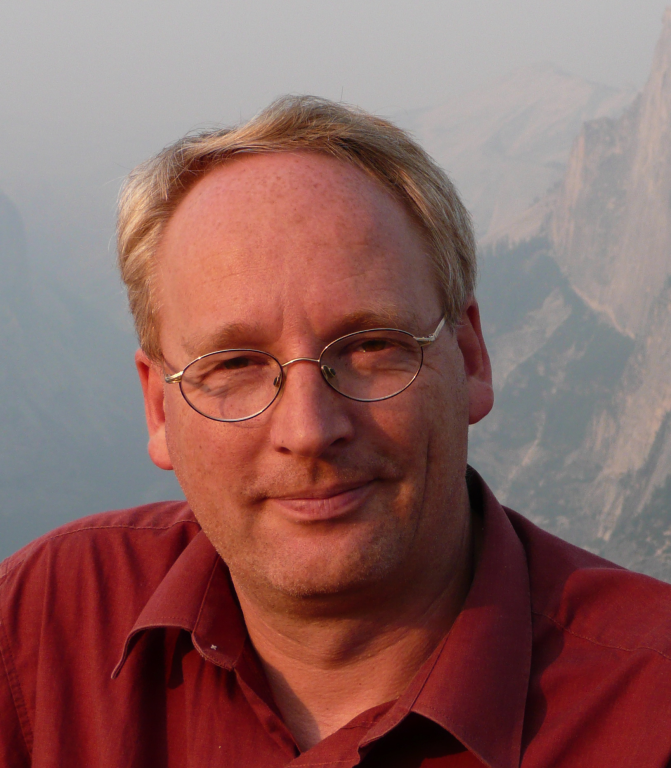
\includegraphics[width=.9\linewidth]{Carsten.png}
\caption{Exemple d'image (au format PNG)}
\end{figure}

\begin{description}
\item[\texttt{C-c C-x C-v}] Inverser l'affichage des images \emph{inline}
\item[\texttt{C-c C-x C-M-v}] Rafraîchir les images
\end{description}
\end{frame}
\subsection{Graphiques}
\label{sec-3-5}

\begin{frame}[fragile,label=sec-3-5-1]{Graphiques R}
 \lstset{language=R,numbers=none}
\begin{lstlisting}
plot(1:10, (1:10)^2)
\end{lstlisting}
\end{frame}
\begin{frame}[fragile,label=sec-3-5-2]{Graphiques R}
 \begin{center}
\begin{tabular}{rr}
1 & 2\\
2 & 4\\
3 & 9\\
4 & 16\\
5 & 25\\
\end{tabular}
\end{center}

\lstset{language=R,label=R-plot,numbers=none}
\begin{lstlisting}
plot(data)
\end{lstlisting}

\begin{verbatim}
nil
\end{verbatim}
\end{frame}
\begin{frame}[fragile,label=sec-3-5-3]{Graphiques Dot}

 \lstset{language=dot,numbers=none}
\begin{lstlisting}
digraph G {
  todo -> done [label="quick", style=dashed];
  todo -> started [label="in progress"]; started -> done;
  todo -> waiting; waiting -> todo;
  todo -> delegated; delegated -> done;
  started [shape=Mdiamond, label="strt"];
  waiting [shape=polygon, sides=5, peripheries=3];
  done [style=bold];
}
\end{lstlisting}

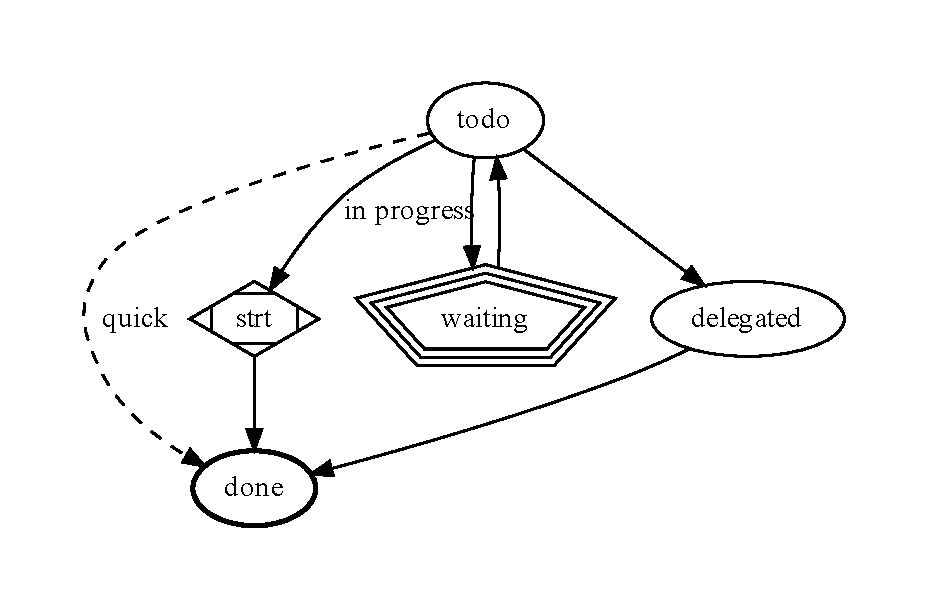
\includegraphics[width=.9\linewidth]{foo.pdf}
\end{frame}
\begin{frame}[fragile,label=sec-3-5-4]{Graphiques TikZ}
 \lstset{language=TeX,numbers=none}
\begin{lstlisting}
\begin{tikzpicture}[scale=1.0]
  \begin{axis}[
    height=7cm, width=10cm,
    ymin=0, % smooth,
    stack plots=y, area style,
    enlarge x limits=false,
    xlabel={Mois}, symbolic x coords={Jan,Fév,Mar,Avr,Mai,Juin,Juil,
      Aoû,Sep,Oct,Nov,Déc},
    xtick=data,
    ylabel={Degrés C},
    title={Températures moyennes à Dunkerque}]
    \addplot coordinates {
      (Jan,3.8) (Fév,4.1) (Mar,6.3) (Avr,9.0)
      (Mai,11.9) (Juin,15.1) (Juil,17.1) (Aoû,17.4)
      (Sep,15.7) (Oct,11.8) (Nov,7.7) (Déc,4.8)}
      \closedcycle;
  \end{axis}
\end{tikzpicture}
\end{lstlisting}
\end{frame}
\begin{frame}[label=sec-3-5-5]{Graphiques TikZ}
\begin{tikzpicture}[scale=1.0]
  \begin{axis}[
    height=7cm, width=10cm,
    ymin=0, % smooth,
    stack plots=y, area style,
    enlarge x limits=false,
    xlabel={Mois}, symbolic x coords={Jan,Fév,Mar,Avr,Mai,Juin,Juil,
      Aoû,Sep,Oct,Nov,Déc},
    xtick=data,
    ylabel={Degrés C},
    title={Températures moyennes à Dunkerque}]
    \addplot coordinates {
      (Jan,3.8) (Fév,4.1) (Mar,6.3) (Avr,9.0)
      (Mai,11.9) (Juin,15.1) (Juil,17.1) (Aoû,17.4)
      (Sep,15.7) (Oct,11.8) (Nov,7.7) (Déc,4.8)}
      \closedcycle;
  \end{axis}
\end{tikzpicture}
\end{frame}
\subsection{Citations}
\label{sec-3-6}

\begin{frame}[fragile,label=sec-3-6-1]{Citations}
 \lstset{language=org,numbers=none}
\begin{lstlisting}
#+begin_quote
,We have seen that computer programming is an art,
,because it applies accumulated knowledge to the world,
,because it requires skill and ingenuity, and especially
,because it produces objects of beauty.
,-- Donald E. Knuth (Communications of the ACM, December 1974)
#+end_quote
\end{lstlisting}

\begin{quote}
We have seen that computer programming is an art,
because it applies accumulated knowledge to the world,
because it requires skill and ingenuity, and especially
because it produces objects of beauty.
-- Donald E. Knuth (Communications of the ACM, December 1974)
\end{quote}
\end{frame}
\subsection{Listings informatiques}
\label{sec-3-7}

\begin{frame}[fragile,label=sec-3-7-1]{Listings informatiques}
 \lstset{language=org,numbers=none}
\begin{lstlisting}
#+BEGIN_SRC sql
,SELECT *
,FROM inventory
,WHERE product IN
,     (SELECT product
,      FROM orders
,      WHERE customer IN ('Pierre','Sarah'));
#+END_SRC
\end{lstlisting}

\lstset{language=SQL,numbers=none}
\begin{lstlisting}
SELECT *
FROM inventory
WHERE product IN
     (SELECT product
      FROM orders
      WHERE customer IN ('Pierre','Sarah'));
\end{lstlisting}
\end{frame}
\subsection{Blocs}
\label{sec-3-8}

\begin{frame}[fragile,label=sec-3-8-1]{Insertion d'environnements \\ Easy templates \texttt{org-structure-template-alist}}
 \begin{itemize}
\item Paires \texttt{\#+BEGIN\_xxx} et \texttt{\#+END\_xxx}
\begin{description}
\item[\texttt{< s TAB}] Insérer un bloc \emph{src}
\item[\texttt{< e TAB}] Insérer un bloc \emph{example}
\item[\texttt{< q TAB}] Insérer un bloc \emph{quote}
\item[\texttt{< v TAB}] Insérer un bloc \emph{verse}
\item[\texttt{< c TAB}] Insérer un bloc \emph{center}
\end{description}
\end{itemize}
\end{frame}
\begin{frame}[fragile,label=sec-3-8-2]{Insertion d'environnements \\ Easy templates \texttt{org-structure-template-alist}}
 \begin{itemize}
\item \LaTeX{}
\begin{description}
\item[\texttt{< l TAB}] Insérer un bloc \emph{latex}
\item[\texttt{< L TAB}] Insérer une directive \emph{latex}
\end{description}

\item HTML
\begin{description}
\item[\texttt{< h TAB}] Insérer un bloc \emph{html}
\item[\texttt{< H TAB}] Insérer une directive \emph{html}
\end{description}

\item ASCII
\begin{description}
\item[\texttt{< a TAB}] Insérer un bloc \emph{ascii}
\item[\texttt{< A TAB}] Insérer une directive \emph{ascii}
\end{description}

\item Autres
\begin{description}
\item[\texttt{< i TAB}] Insérer une directive \emph{index}
\item[\texttt{< I TAB}] Insérer une directive \emph{include}
\end{description}
\end{itemize}
\end{frame}
\begin{frame}[fragile,label=sec-3-8-3]{Verbatim}
 \lstset{language=org,numbers=none}
\begin{lstlisting}
#+begin_verbatim
,L'environnement  verbatim  affiche exactement ce que
,     l'on écrit, e s p a c e s compris!
#+end_verbatim
\end{lstlisting}

\lstset{language=TeX,numbers=none}
\begin{lstlisting}
\begin{verbatim}
L'environnement  verbatim  affiche exactement ce que
     l'on écrit, e s p a c e s compris!
\end{verbatim}
\end{lstlisting}

\begin{verbatim}
L'environnement  verbatim  affiche exactement ce que
     l'on écrit, e s p a c e s compris!
\end{verbatim}
\end{frame}
\begin{frame}[fragile,label=sec-3-8-4]{Commentaire}
 \lstset{language=org,numbers=none}
\begin{lstlisting}
#+begin_comment
Quelques paragraphes qui ne vont pas apparaître dans le PDF.
#+end_comment
\end{lstlisting}

Quelques paragraphes qui ne vont pas apparaître dans le PDF.
\end{frame}
\subsection{Dissertation}
\label{sec-3-9}

\begin{frame}[fragile,label=sec-3-9-1]{Dissertation}
 \lstset{language=org,numbers=none}
\begin{lstlisting}
* Introduction...
* Methodology...
* Findings...
* Conclusion...
* References...
#+LaTeX: \appendix
* Appendix A...
* Appendix B...
\end{lstlisting}

Use the \texttt{\textbackslash{}appendix} command to turn on alphabetic numbering.
\end{frame}
\section{Export \LaTeX{}}
\label{sec-4}

\subsection{Options}
\label{sec-4-1}

\begin{frame}[fragile,label=sec-4-1-1]{Options d'export \\ Quelques options courantes}
 \begin{description}
\item[\texttt{H:3}] \alert{Nombre de niveaux de titre} (sections)
\item[\texttt{num:t}] \alert{Numérotation des sections}
\item[\texttt{toc:t}] \alert{Table des matières} (éventuellement limitée à un @nombre de niveaux@)
\item[\texttt{\textasciicircum{}:nil}] Interprétation des \texttt{\_} et \texttt{\textasciicircum{}} comme \emph{indice} et \emph{exposant}
\end{description}
\end{frame}
\begin{frame}[fragile,label=sec-4-1-2]{Options d'export \\ Quelques options avancées}
 \begin{description}
\item[\texttt{d:nil}] Inclusion des \emph{drawers} (éventuellement limitée à @certains tiroirs@)
\item[\texttt{todo:t}] Inclusion des mots-clés \texttt{TODO}
\item[\texttt{tags:not-in-toc}] Inclusion des \emph{tags} (éventuellement limitée au @titre des
sections@)
\end{description}
\end{frame}
\begin{frame}[fragile,label=sec-4-1-3]{Options d'export \\ \emph{Template} inséré via \texttt{C-c C-e t}}
 \lstset{language=org,numbers=none}
\begin{lstlisting}
#+DESCRIPTION: Tout ce que vous avez toujours voulu savoir sur Org
#+KEYWORDS:  stage, latex, org-mode, dunkerque
#+LANGUAGE:  fr
#+OPTIONS:   H:3 num:t toc:t \n:nil @:t ::t |:t ^:nil -:t f:t *:t <:t
#+OPTIONS:   TeX:t LaTeX:t skip:nil d:nil todo:t pri:t tags:not-in-toc
#+INFOJS_OPT: view:nil toc:nil ltoc:t mouse:underline buttons:0
#+INFOJS_OPT: path:http://orgmode.org/org-info.js
#+EXPORT_SELECT_TAGS: export
#+EXPORT_EXCLUDE_TAGS: noexport
\end{lstlisting}
\end{frame}
\subsection{Commande}
\label{sec-4-2}

\begin{frame}[fragile,label=sec-4-2-1]{Commande interactive}
 \begin{description}
\item[\texttt{C-c C-e} (export)] Afficher le menu d'export
\begin{description}
\item[\ldots{} \texttt{l} (latex)] Exporter en \LaTeX{}
\item[\ldots{} \texttt{p} (process)] \ldots{} et générer le PDF\footnote{Connaître \LaTeX{} est utile en cas d'erreur}
\item[\ldots{} \texttt{d} (display)] \ldots{} et ouvrir le PDF
\end{description}

\item[\texttt{C-c C-e 1} (export)] Limiter l'export au sous-arbre
\end{description}
\end{frame}
\begin{frame}[fragile,label=sec-4-2-2]{Commande batch}
 \begin{itemize}
\item Possibilité d'automatiser la génération d'un PDF via un \verb~Makefile~
\end{itemize}

\lstset{language=sh,numbers=none}
\begin{lstlisting}
EMACS_BATCH = emacs --batch -Q
ORG_FLAGS = --eval "(add-to-list 'load-path \"~/src/org-mode/lisp\")"
ORG_BATCH = $(EMACS_BATCH) $(ORG_FLAGS) -l org-batch-init.el

# Export an Org document to PDF
%.pdf: %.org
	@echo "Exporting $< to PDF..."
	@$(ORG_BATCH) $< -f org-export-as-pdf
	@echo "$@ successfully generated"
\end{lstlisting}
\end{frame}
\section{Avancé}
\label{sec-5}

\subsection{Usages}
\label{sec-5-1}

\begin{frame}[fragile,label=sec-5-1-1]{Usages avancés}
 \begin{itemize}
\item Attacher des \emph{tags} aux sections (et export sélectif)

Cas d'école~: générer un document avec les questions d'examen uniquement, et
un autre avec les questions et les réponses

\item Attacher un statut aux sections (TODO / DONE)

\item Vue \emph{sparse tree} des actions à faire

\item Attacher des dates aux tâches ou événements
\begin{itemize}
\item \texttt{SCHEDULED}
\item \texttt{DEADLINE}
\item \emph{time-stamp} actif
\end{itemize}

\item Vue agenda consolidant les actions et événements de plusieurs fichiers en
une seule vue

\item Calendrier CalFW
\end{itemize}
\end{frame}
\begin{frame}[label=sec-5-1-2]{Usages avancés}
\begin{itemize}
\item Support de \emph{Beamer}

\item Export en ASCII, en HTML et en LibreOffice

\item Mode de capture des actions ou idées

\item Org-Babel

\item \emph{Tracking} du temps passé
\end{itemize}
\end{frame}
\subsection{Crypt}
\label{sec-5-2}

\begin{frame}[fragile,label=sec-5-2-1]{Crypt}
 \begin{itemize}
\item Mots de passe stockés dans le fichier adéquat
\item Cryptage lors de la sauvegarde du fichier
\item \emph{Heading} reste en clair, donc utilisable dans les recherches
\end{itemize}

\lstset{language=org,numbers=none}
\begin{lstlisting}
*** Actions à prendre

*** Mots de passe                                           :crypt:

,- client :: secret
,- serveur :: chuuut!
\end{lstlisting}
\end{frame}
\begin{frame}[fragile,label=sec-5-2-2]{Crypt}
 \lstset{language=org,numbers=none}
\begin{lstlisting}
*** Actions à prendre

*** Mots de passe                                           :crypt:
,-----BEGIN PGP MESSAGE-----
,Version: GnuPG v1.4.12 (Cygwin)

,6BAkIVZDQ6uOYYkNFnG+tPNsObt3DJVQvoR43xNzvjQtqYDSXEcA3bVk3a5341N7
,hp1OszldNgWX5jR9RE6bYri8+57KdXnPbuXFM8wREdTudoXvth66tIud4MjF6UEF
,HyeZ6MfQR2YkEDB1L2ZdeOKLuZZLe+qpxEVskuAQPX2/VydcCBYQufNB52j1APn6
,6pIP0ZWyIa/qvWEfniq+Aqf33OBBQxTtRiXumlXXjacfTcifPnzKUFTvssyf6obr
,oXGATiB8PoThpwqOAmrVNb8no4zVgA5k6D+Lx96WucQNqpsuh4eNMbl0ku5X8nfq
,htJjAV5fbkB2nmxJVWym+dfjhe17xlP2VzmdFCL66rr254zNBNogcAZyney7iJsI
,/ScwsDd2+U19+DXXKHeph1b8r92oE/Z8NKlGshZHVw+laN8a1Bnn6kDaRSHUf+w4
,AqRo44YT
,=zVC2
,-----END PGP MESSAGE-----
\end{lstlisting}

\begin{description}
\item[\texttt{M-x org-decrypt-entry}] Décrypter la section
\end{description}
\end{frame}
\subsection{GTD}
\label{sec-5-3}

\begin{frame}[fragile,label=sec-5-3-1]{Getting Things Done}
 \begin{description}
\item[\texttt{C-c C-q}] Attacher un ou plusieurs \emph{tags}
\item[\texttt{C-c C-t}] Changer le statut
\item[\texttt{C-c C-x t}] Insérer une \emph{inline task} (si paquet \texttt{org-inlinetask} chargé)~:
niveau 15 et suivants

\lstset{language=org,numbers=none}
\begin{lstlisting}
  *************** TODO Faire ceci
  ,Description...
  *************** END
\end{lstlisting}
\end{description}
\end{frame}
\subsection{Agenda}
\label{sec-5-4}

\begin{frame}[label=sec-5-4-1]{Agenda}
Avec tâches répétitives
\end{frame}
\subsection{Autres exports}
\label{sec-5-5}

\begin{frame}[fragile,label=sec-5-5-1]{Autres exports}
 \begin{description}
\item[\texttt{C-c C-e h/b} (html/browser)] Export HTML
\item[\texttt{C-c C-e P} (project)] Site Web
\item[\texttt{C-c C-e o/O} (ODT)] Export LibreOffice
\end{description}
\end{frame}
\subsection{Recherche avancée}
\label{sec-5-6}

\begin{frame}[fragile,label=sec-5-6-1]{Recherche avancée}
 \begin{enumerate}
\item Helm-Imenu (H1 / H2)
\item \texttt{(C-u) C-c C-j}
\item \texttt{C-c a < s *term}
\item \texttt{(C-s) C-o} (occur)
\item \texttt{C-c / / regexp}
\end{enumerate}
\end{frame}
\begin{frame}[fragile,label=sec-5-6-2]{Helm Imenu}
 \begin{itemize}
\item Affichage de tous les \emph{headings} de niveau 1 et 2
\end{itemize}

\lstset{language=org,numbers=none}
\begin{lstlisting}
Introduction / LaTeX
Introduction / Org mode
Structuration / Fichier
Structuration / Packages
Structuration / Titre
Structuration / Sectionnement
\end{lstlisting}

\begin{itemize}
\item Possibilité de limiter la liste avec une \emph{regexp}

\item \texttt{RET} saute sur la section sélectionnée
\end{itemize}
\end{frame}
\subsection{Org-Babel}
\label{sec-5-7}

\begin{frame}[label=sec-5-7-1]{Org-Babel \\ Usages}
\begin{itemize}
\item \emph{Literate Programming} (\emph{LP})

Expliquer la logique du programme dans un langage naturel (tel que le
français), entrecoupé de bouts de code traditionnels

\item Exécution de code

Intégrer des bouts de code exécutable et/ou leurs résultats dans les
documents Org

\item \emph{Reproducible Research} (\emph{RR})

Créer des rapports dynamiques qui peuvent être mis à jour automatiquement si
les données ou l'analyse change
\end{itemize}
\end{frame}
\begin{frame}[fragile,label=sec-5-7-2]{Org-Babel \\ Langages supportés}
 \begin{itemize}
\item \texttt{asymptote}
\item \texttt{awk}
\item \texttt{C++}
\item \texttt{C}
\item \texttt{calc}
\item \texttt{clojure}
\item \texttt{css}
\item \texttt{ditaa}
\item \texttt{dot}
\item \texttt{emacs-lisp}
\item \texttt{gnuplot}
\item \texttt{haskell}
\item \texttt{js}
\item \texttt{latex}
\item \texttt{ledger}
\item \texttt{lilypond}
\item \texttt{lisp}
\item \texttt{matlab}
\item \texttt{mscgen}
\item \texttt{ocaml}
\item \texttt{octave}
\item \texttt{org}
\item \texttt{perl}
\item \texttt{plantuml}
\item \texttt{python}
\item \texttt{R}
\item \texttt{ruby}
\item \texttt{sass}
\item \texttt{scheme}
\item \texttt{screen}
\item \texttt{sh}
\item \texttt{sql}
\item \texttt{sqlite}
\end{itemize}
\end{frame}
\begin{frame}[fragile,label=sec-5-7-3]{Org-Babel \\ Exécution de code --- Usages}
 \begin{itemize}
\item Manuel d'opérations "exécutable"
\begin{itemize}
\item \texttt{cd <dir>}
\item \texttt{ls}
\item \texttt{cp <file>}
\item \texttt{grep}
\end{itemize}

\item Transformation de données brutes en observations

\item Génération de code \LaTeX{} (en Elisp ou n'importe quel autre langage) avec le
paramètre d'output \texttt{:results latex}
\end{itemize}
\end{frame}
\begin{frame}[fragile,label=sec-5-7-4]{Org-Babel \\ Exécution de code --- Code en ligne}
 \begin{itemize}
\item Org

\lstset{language=org,numbers=none}
\begin{lstlisting}
,  En Calc, 1 + 2 = src_calc{1+2}.

,  En R, 2 + 3 = src_R[:results raw]{2+3}.
\end{lstlisting}

\item \LaTeX{}

\lstset{language=TeX,numbers=none}
\begin{lstlisting}
  En Calc, 1 + 2 = \texttt{3}.

  En R, 2 + 3 = 5.
\end{lstlisting}

\item PDF

En Calc, 1 + 2 = \texttt{3}.

En R, 2 + 3 = 5
\end{itemize}
.
\end{frame}
\begin{frame}[fragile,label=sec-5-7-5]{Org-Babel \\ Exécution de code --- Code hors ligne}
 \begin{itemize}
\item Org
\end{itemize}

\lstset{language=org,numbers=none}
\begin{lstlisting}
#+BEGIN_SRC emacs-lisp :exports code
,(message "%s" "hello world")
#+END_SRC
\end{lstlisting}

\begin{itemize}
\item \LaTeX{}
\end{itemize}

\lstset{language=TeX,numbers=none}
\begin{lstlisting}
\begin{verbatim}
 hello world
\end{verbatim}
\end{lstlisting}

\begin{itemize}
\item PDF
\end{itemize}

\begin{verbatim}
hello world
\end{verbatim}
\end{frame}
\begin{frame}[label=sec-5-7-6]{Librairie de Babel}
\begin{itemize}
\item Manipulation de tables
\begin{itemize}
\item Filtrage
\item Transposition
\item Affichage à l'export
\end{itemize}

\item Graphiques

\item \ldots{}
\end{itemize}
\end{frame}
\begin{frame}[fragile,label=sec-5-7-7]{Exécution de code \\ SQL}
 \lstset{language=org,numbers=none}
\begin{lstlisting}
#+name: top-5-dossiers
#+BEGIN_SRC sql
,SELECT TOP 5 prsPfiID_fk, COUNT(*) AS 'Nb Prestations'
,FROM prestations
,GROUP BY prsPfiID_fk
,ORDER BY COUNT(*) DESC
#+END_SRC

#+results: top-5-dossiers
,| prsPfiID_fk    | Nb Prestations |
,|----------------+----------------|
,| 73/200509/0111 |             22 |
,| 52/200302/0047 |             21 |
,| 61/200604/0007 |             21 |
,| 62/200312/0052 |             20 |
,| 72/200511/0016 |             20 |
\end{lstlisting}
\end{frame}
\subsection{Time clocking}
\label{sec-5-8}

\begin{frame}[label=sec-5-8-1]{Time clocking \\ Track time}
\#+BEGIN\_SRC org :exports code
\end{frame}

\subsection{{\color{red}\textbf{\textsc{\textsf{TODO}}}} Laver les fenêtres à l'étage}
\label{sec-5-9}
\#+END\_SRC

\begin{description}
\item[\texttt{C-c C-x e} (effort)] Donner une estimation du temps de travail
\item[\texttt{C-c C-x C-i} (in)]
\item[\texttt{C-c C-x C-j} (jump)]
\item[\texttt{C-c C-x C-o} (out)]
\end{description}
\section{Installation}
\label{sec-6}

\subsection{Installation}
\label{sec-6-1}

\begin{frame}[fragile,label=sec-6-1-1]{Installation du système}
 \begin{itemize}
\item Version récente livrée avec \alert{Emacs}

\lstset{language=Lisp,numbers=none}
\begin{lstlisting}
  M-x org-version
\end{lstlisting}

\item Dernière version stable (\verb~7.8.11~) sur \url{http://orgmode.org/}

\item Version de développement via Git

\lstset{language=sh,numbers=none}
\begin{lstlisting}
  git clone git://orgmode.org/org-mode.git
  cd org-mode
  make autoloads
\end{lstlisting}

\begin{itemize}
\item You need to ``make autoloads'' after pulling. That will remake
org-version.el and org-install.el to reflect reality.

\item or make uncompiled?
\end{itemize}
\end{itemize}
\end{frame}
\subsection{Sources d'informations}
\label{sec-6-2}

\begin{frame}[label=sec-6-2-1]{Sources d'informations}
\begin{itemize}
\item Manuels de référence
\begin{itemize}
\item \href{http://orgmode.org/orgcard.pdf}{Org mode Reference Card} (2 pages)
\item \href{http://orgmode.org/orgguide.pdf}{The compact Org mode Guide} (\textpm{} 40 pages)
\item \href{http://orgmode.org/org.pdf}{The Org Manual} (\textpm{} 250 pages)
\end{itemize}

\item \href{http://orgmode.org/worg/org-faq.html}{FAQ Org mode}

\item Site \href{http://orgmode.org/worg/}{Worg} (= Wiki sur Org mode)
\begin{itemize}
\item Écrit en Org
\item Publié en HTML
\end{itemize}

\item Site \href{http://www.emacswiki.org/emacs/OrgMode}{EmacsWiki}

\item Liste de discussion \href{mailto:emacs-orgmode@gnu.org}{emacs-orgmode@gnu.org}

\item Exemples de documents académiques rédigés en Org
\begin{itemize}
\item \href{http://www.jstatsoft.org/v46/i03}{Article publié au Journal of Statistical Software}
\end{itemize}
\end{itemize}
\end{frame}
\section{Conclusions}
\label{sec-7}

\subsection{Conclusions}
\label{sec-7-1}

\begin{frame}[fragile,label=sec-7-1-1]{Approches}
 \begin{itemize}
\item Org pour tout
\item \LaTeX{} si pas de Babel
\item \LaTeX{} avec \texttt{comment} pour l'édition de tables
\end{itemize}
\end{frame}
\begin{frame}[label=sec-7-1-2]{Avantages}
\begin{itemize}
\item \alert{Séparation fond -- forme(s)}
\begin{itemize}
\item Concentrez-vous sur le contenu~!
\item Org mode vous le permet via sa syntaxe allégée et sa facilité d'édition
\item Si des choses doivent être fixées, faites-le à la fin (éventuellement, en
le mettant en \LaTeX{} directement dans le fichier Org)
\end{itemize}

\item \alert{Une seule source}
\begin{itemize}
\item Données brutes
\item Notes privées (mots de passe, rêveries, etc.)
\item Analyses (bouts de code)
\item Résultats
\item \emph{Inline tasks} pour la gestion de tâches
\end{itemize}

\item Exporter
\begin{itemize}
\item Vers différents formats
\item Uniquement les parties que l'on veut exporter
\end{itemize}
\end{itemize}
\end{frame}
\begin{frame}[label=sec-7-1-3]{Questions~?}

\includegraphics[width=.9\linewidth]{questions.png}
\end{frame}
\section{Remerciements}
\label{sec-8}

\subsection{Remerciements}
\label{sec-8-1}

\begin{frame}[label=sec-8-1-1]{Remerciements}
Merci à Denis Bitouzé de m'avoir permis (d'essayer) de vous contaminer~!


\includegraphics[width=.9\linewidth]{thank-you-all-languages.png}
\end{frame}
% Emacs 24.3.1 (Org mode 8.0.3)
\end{document}
